\chapter{Braking levels for automated vehicles}
\label{A:brake}
Three levels of brake for the automated vehicles are defined in our VR experiment as follows:
\begin{itemize}
    \item \textbf{Level 1}: given the initial speed of the vehicle when observing the pedestrian ($V_0$) and its corresponding distance to the pedestrian ($d$), \textit{one} constant deceleration rate is calculated to stop the car before the pedestrian and avoid a collision. A maximum possible deceleration rate is set to be $a_{max} = -3 m/s^2$. Thus, if the calculated acceleration rate surpasses the maximum possible rate, the vehicle stops with the rate of $a_{max}$, but cannot stop for the pedestrian completely in a timely manner. 
    \item \textbf{Level 2:} given the initial speed of the vehicle when observing the pedestrian ($V_0$) and its corresponding distance to the pedestrian ($d$), \textit{two} constant deceleration rates are calculated $a_1$ and $a_2$. $a_1$ changes the speed of vehicle from $V_0$ to $V_0/2$ in $d/2$ of the distance, and $a_2$ decreases the speed from there to stop in the rest $d/2$ of distance. Similar to level 1, deceleration rate cannot exceed $a_{max}$ in neither of the two steps. 
    \item \textbf{Level 3:} given the initial speed of the vehicle when observing the pedestrian ($V_0$) and its corresponding distance to the pedestrian ($d$), \textit{three} constant deceleration rates are calculated: $a_1$, $a_2$, and $a_3$. $a_1$ changes the speed of vehicle from $V_0$ to $2V_0/3$ in the first $d/3$ of the distance, $a_2$ decreases the speed from there to $V_0/3$ in the next $d/3$ of the distance, and $a_3$ stops the vehicle in the final $d/3$ of distance. Similar to level 1 and 3, deceleration rate cannot exceed $a_{max}$ in none of the steps. 
\end{itemize}
Based on the definitions provided, the speed-distance profile of the braking levels is drawn for three scenarios:
\begin{itemize}
    \item \textbf{Scenario 1:} $V_0 = 40 km/hr$, $d = 40 meters$ 
    
     \item \textbf{Scenario 2:} $V_0 = 50 km/hr$, $d = 40 meters$ 
     
     \item \textbf{Scenario 3:} $V_0 = 50 km/hr$, $d = 20 meters$ 
\end{itemize}

In scenario 1, the vehicle with level 1 braking system manages to decelerate and stop the car right before a barrier seen in 40 meters, whereas the two other braking levels stop the vehicle a few meters before the barrier. As the initial speed increases to 50 km/hr in scenario 2, level 2 and level 3 also take longer distance to stop the car, although the speed of the vehicle is slower when it is close to the barrier, generating a more smooth experience for the pedestrian. In scenario 3, however, not enough distance exists between the barrier and the vehicle. The 20 meter distance makes all the braking levels at all their steps to perform at $a_{max}$, making all similar profiles for all the levels. The speed profile of the three aforementioned scenarios are presented in \cref{fig:prof}.
\begin{figure}[!t]
\begin{adjustbox}{varwidth=\textwidth,fbox,center}
\centering
\begin{subfigure}{0.95\linewidth}

    \begin{subfigure}[b]{0.45\textwidth}
         \centering
         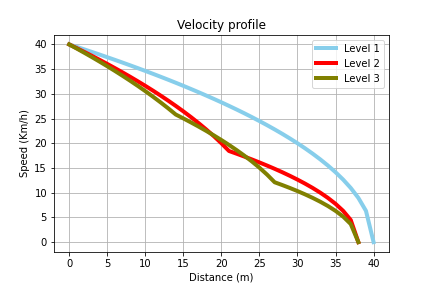
\includegraphics[scale=0.4]{appendix/figures/r40_40.png}
         \caption{Initial speed: 40 km/hr, initial distance: 40 m}
     \end{subfigure}
     \hfill
     \begin{subfigure}[b]{0.45\textwidth}
         \centering
         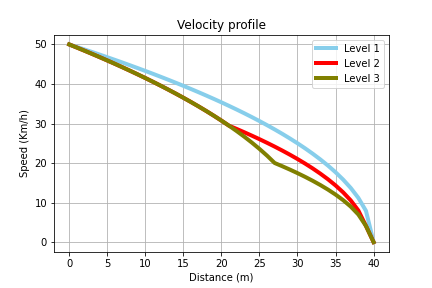
\includegraphics[scale=0.4]{appendix/figures/r40_50.png}
         \caption{Initial speed: 50 km/hr, initial distance: 40 m}
     \end{subfigure}
\end{subfigure}\\[2ex]
\begin{subfigure}{0.8\linewidth}

\centering
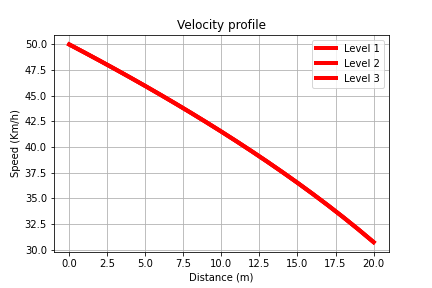
\includegraphics[scale=0.4]{appendix/figures/r20_50.png}
\caption{Initial speed: 50 km/hr, initial distance: 20 m}

\end{subfigure}
\end{adjustbox}
\caption{Velocity profile for three hypothetical scenarios}
\label{fig:prof}
\end{figure}

